%% References
%% https://alexanderfabisch.github.io/latex-for-dissertations.html

\documentclass[
    draft=false,
    paper=a4,
    % twoside, % twoside is default for scrbook
    paper=portrait,
    pagesize=auto,
    fontsize=11pt,
    DIV=calc, % DIV value as calculated from paper and font size
    BCOR=15mm, % binding correction
    titlepage=firstiscover, % print title page as cover
    version=last,
    headings=twolinechapter,
    listof=totoc,
    listof=chapterentry]{scrbook}

\setkomafont{disposition}{\rmfamily\scshape}
\setkomafont{publishers}{\large}

\usepackage{libertinus}

\usepackage{scrhack} % fix a few common issues with KOMA-classes


% Citation Management
\usepackage[
    style=authoryear-comp, % citation style
    natbib=true,
    backend=biber,
    maxnames=2,
    maxbibnames=99]{biblatex}
\addbibresource{literature.bib}

% while drafting
% \includeonly{chapters/introduction}
\setlength{\marginparwidth }{2cm} 
\usepackage[obeyDraft]{todonotes}
\setuptodonotes{inline}
% FOR TESTING
\usepackage{blindtext}
% \usepackage{showframe}


\usepackage[ngerman, english]{babel} %last language in the list is the main language, in this case English (American)
% font as needed for additional languages


% CJK support
\usepackage{xeCJK}
\setCJKmainfont{Noto Serif CJK TC}
\setCJKsansfont{Noto Sans CJK TC}
\setCJKmonofont{Noto Sans Mono CJK TC}

% quotation style
\usepackage[english=american]{csquotes}


% \usepackage{amsmath}
% \usepackage{amssymb}

% other
\usepackage{microtype}
\usepackage{graphicx}
\usepackage{hyperref}
\usepackage{caption}
\usepackage{subcaption}
\usepackage{tabularx}
\usepackage{longtable}
\usepackage{booktabs}
\usepackage{lscape}
\usepackage{rotating}
\usepackage{adjustbox}
% \newtheorem{definition}{Definition}
% \newtheorem*{definition*}{Definition}

% linguistics stuff
\usepackage{tikz-dependency}
\usepackage{forest}
\usepackage{gb4e}
\noautomath

\begin{document}

% title information
\titlehead{{\Large Saarland University\\}
    {Department of Language Science and Technology}\\
    Faculty of Humanities}
\subject{Master's Thesis}
\title{Typological investigations of verbal valency systems}
\subtitle{A quantitative study based on Universal Dependencies}
\author{Siyu Tao}
\date{\today}
\publishers{
    \begin{tabular}{rl}
        Advisors:& Prof. Dr. Michael Hahn\\
        {}& Dr. Lucia Donatelli\\
        {}&{}\\
        Supervisors: & Jun.-Prof. Dr. Annemarie Verkerk\\
        {}& Dr. Lucia Donatelli
    \end{tabular}\\
    \vspace{5cm}
    
\includegraphics[height=2cm]{figures/UdS_Logo.pdf}
}

% Title page and front matter
\frontmatter
\maketitle
\addchap*{}
\begin{center}
    \bfseries \Large
    Eidesstattliche Erklärung
\end{center}
    Hiermit erkläre ich,
    dass ich die vorliegende Arbeit selbstständig verfasst und keine anderen als die angegebenen Quellen und Hilfsmittel verwendet habe.
    Ich versichere,
    dass die gedruckte und die elektronische Version der Masterarbeit inhaltlich übereinstimmen.
\begin{center}
    \bfseries\itshape \Large
    Statutory Declaration
\end{center}
{
\itshape
I hereby declare that
the thesis presented here is my own work and that no other sources or aids, other than those listed, have been used.
I affirm that the electronic version is identical in content to the printed version of the Master's thesis.}
  \vfill
  \vfill
  Ort, Datum / \textit{Place, date}:\\
  \rule[1em]{25em}{0.5pt}  % This prints a line to write the date

  Unterschrift / \textit{Signature}:\\
  \rule[1em]{25em}{0.5pt}  % This prints a line for the signature

\addchap*{Acknowledgments}

\addchap{Abstract}
\blindtext
 
\tableofcontents

\mainmatter
\chapter{Introduction}

Universal Dependencies (UD) treebanks, a multilingual collection of dependency treebanks based on a shared, cross-lingually consistent annotation scheme \citep{nivre2020} and covering 138 languages with 243 treebanks in its most recent \texttt{v2.11} release \citep{universaldep}, have enabled significant advances in the development of multilingual dependency parsers and other NLP technologies \citep{zeman2017, zeman2018}. This proposed thesis will explore their potential in typology research through a cross-lingual quantitative study of verbal valency systems.

The starting point of this study is the assumption, consistent with those behind \citet{levin1993} and other work on \textit{verb classes}, that the syntactic behavior of verbs are at least in part determined by their lexical semantics, and that, as such, verb classes based on their syntactic distribution should be semantically coherent as well. This study will test this assumption computationally by performing clustering experiments on a subset of UD treebanks in order to explore whether the UD annotations support an automated induction of the valency frames in a language and whether verb classes can be further inducted based on the distribution of verbs across the valency frames. In the process of the experiments, factors that have an impact on the outcome of clustering, particularly with respect to data quantity and quality, as well as typological features of languages, will be examined. The results of these clustering experiments will then, in combination with a computationally derived cross-lingual lexicon, support typological investigations into possible universals in the organization of verbal lexicon.

We develop a quantitative methodology. The methodology is described along with experiment design in the respective sections.
\chapter{Background and theoretical framework}\label{chapter:background}
\section{Valency and valency phenomena}

% valency - terminology introduction

In chemistry, \textit{valency}, or \textit{valence}, refers to the combining power of an atom or radical. The valency of any atom can be measured by the number of hydrogen atoms that it can combine with or displace in a chemical compound \citep{law2020a}. This same term was introduced to linguistics by analogy and refers to the combining power of a word, primarily a verb or predicate, with other words or elements of the sentence. 

Lucien Tesnière is generally credited with introducing the term valency to linguistics with his syntactic theory of valency and dependence, as presented in the posthumously published \textit{Éléments de syntaxe structurale} (\cite*{tesniere1959}; English translation \cite*{tesniere2015}).\footnote{
    It should be noted that while Tesnière is rightly credited with the introduction of a theory of linguistic valency, the metaphor of valency itself has made appearances as early as in \citet{peirce1897}, among others \citep{przepiorkowski2018}.
}
In another of Tesnière's analogies, each verbal node, being the center of sentence structure, is not unlike a ``theatrical performance'' with the verb expressing the process and the nouns being the \textit{actants} (what we would now call \textit{arguments}) in this performance. Just like how atoms of different elements allow for a greater or lesser number of bonds, different verbs can combine with a greater or lesser number of actants, i.e., their valency.

% the phenomena now we are now calling valency - different theories
While the term valency is borrowed into linguistics from chemistry, the study of the phenomena which are covered by or otherwise overlap with valency has a much longer tradition, dating to the early beginnings of linguistics from the kāraka concept of semantic relation between verb and noun \citep{ganeri2011a} in Pāṇinian grammar to modern case grammar \citep{fillmore1968}. 

Implicit in the focus on verbal valency is the assumption, shared by most linguistic theories, of the centrality of the verb in determining either or both the syntactic and semantic structure of a sentence. This assumption has also been corroborated by psycholinguistic evidence \citep{healy1970} and places valency and the issues of \textit{argument structure} squarely at the center of the inquiry into the interface between syntax and lexical semantics.

%% subcategorization in generative grammar
In generative grammar, the syntactic valency of a verb is treated under a similar notion of \textit{subcategorization} \citep{chomsky1965a}. As an example, a transitive verb must be followed by a direct object, whereas an intransitive verb cannot. As such, transitive and intransitive verbs form subcategories of the category of verb. Verbs are thus further assigned to \textit{subcategorization frames} which specify the number and type of complements, i.e., objects and obliques, (and of subjects as well in later theories), that the verb can be subcategorized for. In addition to being syntactically driven, a notable feature of generative theories' treatment of valency is that the subcategorization frames are considered as part of the lexical entry of the verb. Later work in generative grammar, in particular \citet{jackendoff1972,jackendoff1987,jackendoff1992}, following \citet{katz1963} and \citet{gruber1962}, further developed a theory of thematic relations and posited that argument structure serves as the interface between syntactic and thematic structures.
% unclear on relationship between subcategorization and selection in generative grammar; also maybe more citations and examples here later

%% Levin
As compared to broader distinctions such as those made between transitive and intransitive verbs, \citet{levin1993} categorized verbs in a much more fine-grained manner based on their syntactic behavior into different verb classes. Starting from the assumption that the syntactic behavior of verbs are determined semantically, Levin reasons that patterning together classes of verbs based on their diathesis alternations should result in semantically coherent verb classes. Levin's work has been highly influential both in the development of valency theory, where it spurred further work on verb classes, and in computational approaches to lexical semantics, where the VerbNet \citep{kipper-schuler2005, kipper2006, kipper2008} is a prominent example of projects extending the Levin verb classes into a computational lexicon that links with other resources such as WordNet \citep{fellbaum1998, miller1995}, PropBank \citep{kingsbury2002}. Further work on verb class induction based on syntactic patterns includes \citet{basili1993, navarretta2000, korhonen2006, sun2008, sun2009,sun2013} in English, \citet{schulteimwalde2002, schulteimwalde2003, schulteimwalde2006} in German, \citet{snider2006} in Arabic. \citet{sun2013} in particular included diathesis alternation as input feature. Other work focused instead on the induction of semantic verb classes such as \citet{furstenau2012, majewska2018, majewska2020}. And work such as \citet{dowty1991, abend2009, titov2012, bickel2014, sayeed2018, watanabe2010, yamada2021}, among others, worked on the induction of semantic roles, a topic arguably tightly related to the induction of the verb classes.
 
%% frame semantics - fillmore
Another computational project focused on verbal valency, FrameNet \citep{baker1998, fillmore2015} differs from VerbNet in terms of their theoretical foundations, in that it derives from a divergent line of research that stemmed from Charles Fillmore's frame semantics \citep{fillmore1977, fillmore1977a, fillmore1982}, which in turn has its roots in his earlier work on case grammar \citep{fillmore1968,fillmore1970}. While they are often computationally interoperable to some extent, there remains a key conceptual distinction made in frame semantics \citet{fillmore1968}, namely the \textit{frames}-driven analysis of argument encoding. While the verbal lexicon continues to play a role in placing selectional restrictions on the frames in which a given verb can be found in, the frames are themselves said to have semantics through their grouping of frame elements, which are similar to thematic roles but local to their specific frames. The frame semantics approach is consolidated by further development in construction grammar where the frames are viewed as a level of constructions on their own, cf. e.g., \citet{goldberg1992,goldberg1995}'s \textit{argument structure constructions}. Furthermore, construction grammar theories often argue for frames to be considered distinct or autonomous constructions, as it is not strictly predictable from other constructions.

\section{Typological perspectives on valency and dependency}

It is perhaps not surprising that, besides introducing the analogy of valency, \citet{tesniere1959} also introduced the notion of dependency into modern linguistics. In terms of their mathematical foundations, dependency grammar, based on the notion of dependencies, can be viewed in contrast with constituency grammars which are based on the notion of substitution instead \citep{stabler2019}. However, even most iterations of generative grammar theories, which are primarily constituency-based, incorporate some version of a head-dependent relationship (cf. X-bar theory). \citet{demarneffe2019} cited the easiness of generalization across languages, its operationalization of human sentence processing facts, and the transparency and simplicity of representation as reasons why dependency-based representations have become increasingly widely adopted in linguistic theory and even more so in NLP.

The usefulness of dependency grammar in allowing for cross-lingual generalizations and comparisons of linguistic structures should not be understated. Universal Dependencies (UD) \citep{nivre2015,demarneffe2021} in particular is an initiative that aims to develop a uniform grammatical annotation system that are cross-lingually consistent. The basic structure of the UD annotation is to segment \textit{sentences} into \textit{syntactic words} which are annotated with their \textit{morphological properties} and linked together by \textit{syntactic relations}. A comparison of UD annotations of equivalent sentences in two languages shows how they can show both the structural parallel and differences between how two languages encode the same sentence, as seen in Fig.~\ref{fig:ud-example-sentence}, where both the similarities between how English and Finnish encoded semantically equivalent sentences (same syntactic relationships between the arguments and the verb) and the differences (case markings in Finnish, preposition in English) are easily discernable. And further enhancements have also been proposed that would make the UD annotation scheme more compatible with contemporary typological theory \citep{croft2017}.

\begin{figure}
    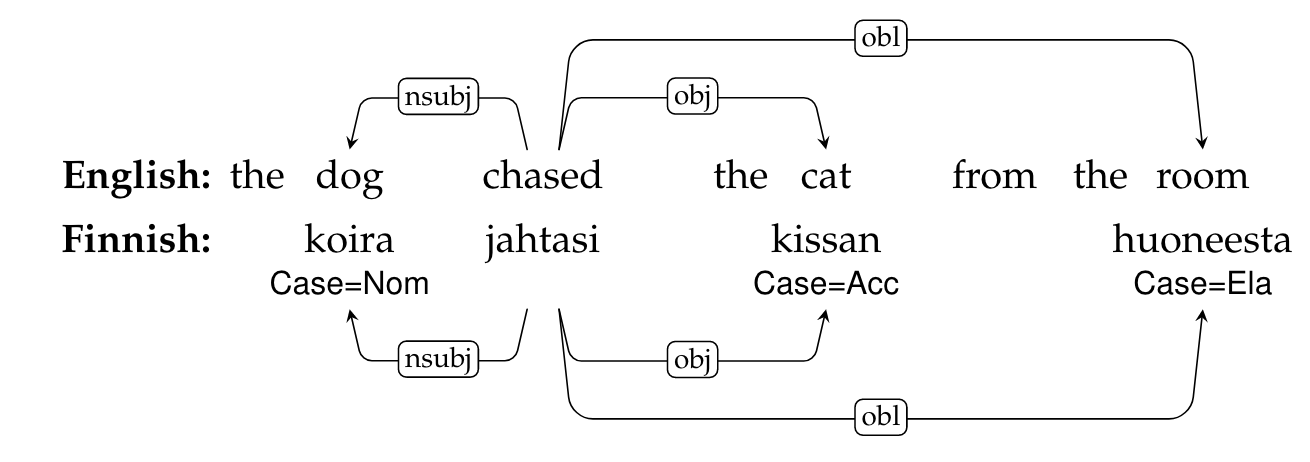
\includegraphics[width=0.85\textwidth]{figures/ud_example_sentence.png}
    \centering
    \caption{Simplified UD annotation for equivalent sentences from English (top) and Finnish (bottom) \citep{demarneffe2021}.}\label{fig:ud-example-sentence}
\end{figure}

Specifically on verbal valency, already \citet{tesniere1959} was paying attention to the cross-lingual differences in the argument structure of semantically equivalent sentences while describing his dependency grammar. Tesnière described the process of \textit{metataxis}, by which syntactic structures of one language are ``translated'' to those of another. Such a process points to the clear typological interest in valency systems, namely the mismatch between how languages encode their argument structure.

\todo{transitivity}

% focus on markedness hierarchy
In terms of possible universals that can be observed, \citet{tsunoda1981, tsunoda1985} proposed a transitivity hierarchy of verbs:
\begin{quote}
    Effective action >> Perception >> Pursuit >> Knowledge >> Feeling >> Relation
\end{quote}
The idea is that languages that encode verbs that are lower in this hierarchy as transitive verbs will encode all those above them too as transitive, with the effective action being the most prototypical transitive verb, hence most likely to be transitive in a language. This approach is further extended by \citet{malchukov2005} who used the semantic map method and proposed a two-dimensional transitivity hierarchy with the semantic map method. 

There has been some recent work from advocates of both the lexeme- and frames-based approaches on the cross-lingual alignment of their respective units of linguistic analysis. On the frames-based side, \citet{baker2020, ellsworth2021} explored the cross-lingual alignment of frames based on FrameNet; in contrast, \citet{say2014} rejected the equating of minor valency classes cross-lingually and studied how verb classes compare cross-lingually instead, seeing that as a more valid method of measuring how languages organize their verbal lexicon differently.

\chapter{Data selection}

\section{Data sources}\label{sec:data}

\subsection{Universal Dependencies}\label{subsec:data_ud}


\textbf{Universal Dependencies (UD)} is the main source of primary data used for the present study. It is designed to be a cross-linguistically consistent system for annotating morphosyntactic information within a dependency grammar framework \citep{demarneffe2021}. 

The v2 update to the UD annotation guidelines also introduced changes that intend to decrease the reliance on language-specific categories \citep{nivre2020}. Inevitably, these efforts had to be balanced against the practicality of computational efficiency but nevertheless converged in many cases with proposals by typologists, as the core principles converged with a functional typology approach. \citet{croft2017}

\begin{enumerate}
    \item UD needs to be satisfactory on linguistic analysis grounds for individual languages.
    \item UD needs to be good for linguistic typology, i.e., providing a suitable basis for bringing out cross-linguistic parallelism across languages and language families.
    \item UD must be suitable for rapid, consistent annotation by a human annotator.
    \item UD must be easily comprehended and used by a non-linguist, whether a language learner or an engineer with prosaic needs for language processing. We refer to this as seeking a \textit{habitable} design, and it leads us to favor traditional grammar notions and terminology.
    \item UD must be suitable for computer parsing with high accuracy.
    \item UD must support well downstream language understanding tasks (relation extraction, reading comprehension, machine translation, \dots).
\end{enumerate}

The \textbf{Universal Dependencies} treebanks \citep{universaldep} is the collection of cross-lingual treebanks annotated in the UD framework by an open community of more than 300 contributors. See \ref{tab:treebanks} for a table of languages available in UD v2.5, as an example.

\begin{table}[t]{}
    \centering
\begin{adjustbox}{center,scale=0.85}
\footnotesize
\renewcommand{\tabcolsep}{3pt}
    \begin{tabular}{|lrrr|lrrr|lrrr|}
    \hline
    \textbf{Language}  & \textbf{\#} & \textbf{Sents} & \textbf{Words} & \textbf{Language}  & \textbf{\#} & \textbf{Sents} & \textbf{Words} & \textbf{Language}  & \textbf{\#} & \textbf{Sents} & \textbf{Words} \\
    \hline
Afrikaans &1 &1,934 &49,276 &German &4 &208,440 &3,753,947 &Old Russian &2 &17,548 &168,522 \\
Akkadian &1 &101 &1,852 &Gothic &1 &5,401 &55,336 &Persian &1 &5,997 &152,920 \\
Amharic &1 &1,074 &10,010 &Greek &1 &2,521 &63,441 &Polish &3 &40,398 &499,392 \\
Ancient Greek &2 &30,999 &416,988 &Hebrew &1 &6,216 &161,417 &Portuguese &3 &22,443 &570,543 \\
Arabic &3 &28,402 &1,042,024 &Hindi &2 &17,647 &375,533 &Romanian &3 &25,858 &551,932 \\
Armenian &1 &2502 &52630 &Hindi English &1 &1,898 &26,909 &Russian &4 &71,183 &1,262,206 \\
Assyrian &1 &57 &453 &Hungarian &1 &1,800 &42,032 &Sanskrit &1 &230 &1,843 \\
Bambara &1 &1,026 &13,823 &Indonesian &2 &6,593 &141,823 &Scottish Gaelic &1 &2,193 &42,848 \\
Basque &1 &8,993 &121,443 &Irish &1 &1,763 &40,572 &Serbian &1 &4,384 &97,673 \\
Belarusian &1 &637 &13,325 &Italian &6 &35,481 &811,522 &Skolt S\'ami &1 &36 &321 \\
Bhojpuri &1 &254 &4,881 &Japanese &4 &67,117 &1,498,560 &Slovak &1 &10,604 &106,043 \\
Breton &1 &888 &10,054 &Karelian &1 &228 &3,094 &Slovenian &2 &11,188 &170,158 \\
Bulgarian &1 &11,138 &156,149 &Kazakh &1 &1,078 &10,536 &Spanish &3 &34,693 &1,004,443 \\
Buryat &1 &927 &10,185 &Komi Permyak &1 &49 &399 &Swedish &3 &12,269 &206,855 \\
Cantonese &1 &1,004 &13,918 &Komi Zyrian &2 &327 &3,463 &Swedish Sign Language &1 &203 &1,610 \\
Catalan &1 &16,678 &531,971 &Korean &3 &34,702 &446,996 &Swiss German &1 &100 &1,444 \\
Chinese &5 &12,449 &285,127 &Kurmanji &1 &754 &1,0260 &Tagalog &1 &55 &292 \\
Classical Chinese &1 &15,115 &74,770 &Latin &3 &41,695 &582,336 &Tamil &1 &600 &9,581 \\
Coptic &1 &1,575 &40,034 &Latvian &1 &13,643 &219,955 &Telugu &1 &1,328 &6,465 \\
Croatian &1 &9,010 &199,409 &Lithuanian &2 &3,905 &75,403 &Thai &1 &1,000 &22,322 \\
Czech &5 &127,507 &2,222,163 &Livvi &1 &125 &1,632 &Turkish &3 &9,437 &91,626 \\
Danish &1 &5,512 &100,733 &Maltese &1 &2,074 &44,162 &Ukrainian &1 &7,060 &122,091 \\
Dutch &2 &20,916 &306,503 &Marathi &1 &466 &3,849 &Upper Sorbian &1 &646 &11,196 \\
English &7 &35,791 &620,509 &Mby\'a Guaran\'i &2 &1,144 &13,089 &Urdu &1 &5,130 &138,077 \\
Erzya &1 &1,550 &15,790 &Moksha &1 &65 &561 &Uyghur &1 &3,456 &40,236 \\
Estonian &2 &32,634 &465,015 &Naija &1 &948 &12,863 &Vietnamese &1 &3,000 &43,754 \\
Faroese &1 &1,208 &10,002 &North S\'ami &1 &3,122 &26,845 &Warlpiri &1 &55 &314 \\
Finnish &3 &34,859 &377,619 &Norwegian &3 &42,869 &666,984 &Welsh &1 &956 &16,989 \\
French &7 &45,074 &1,157,171 &Old Church Slavonic &1 &6,338 &57,563 &Wolof &1 &2,107 &44,258 \\
Galician &2 &4,993 &164,385 &Old French &1 &17,678 &170,741 &Yoruba &1 &100 &2,664 \\
\hline
    \end{tabular}
\end{adjustbox}
    \caption{Languages in UD v2.5 with number of treebanks (\#), sentences (Sents) and words (Words) \citep{nivre2020}.}
    \label{tab:treebanks}
\end{table}

The thesis uses the UD v2.11 release.

In additional to the main data source of UD treebanks, additional resources will be used in the study as reference and to perform validation and evaluation of the intermediate results. As an example, the valency frames and verb classes as induced from the UD treebanks will be validated, where possible, against the expert-annotated data from \textbf{the Valency Patterns Leipzig Online Database (ValPaL)} \citep{valpal}. Other datasets will be introduced as necessary.

\section{Representing verb instances}

In the first step, the specific uses of verbs are abstracted through a feature selection process. Each instance of verb use will be represented by the morphosyntactic features of the sentence, namely only features that are considered part of valency frame encoding are included. This is in order to focus on whether semantically coherent verb classes can be induced from valency frame information alone. In selecting the features, cross-lingual differences in valency frame coding will be taken into account, e.g., whether a language uses morphological cases or word order to encode valency frame information. Word order information, although not explicitly specified in UD, should also be extracted from the dataset. An alternative approach considered is to keep manual feature selection at a minimum and to allow the clustering algorithms to weigh the features as needed.

\section{Clustering}

The clustering process after feature selection consists of two steps, but the clustering algorithms used need not be the same. The first is the automatic induction of valency frames in a language given the selected features and the second is the clustering of verbs, represented by their distribution over the valency frames, into verb classes. Since unsupervised clustering will be used, the number of valency frames and the number of verb classes cannot be assumed \textit{a priori}. This requires either using algorithms that do not require a predefined number of clusters (e.g., Ward clustering), or experimenting with cluster sizes with each language (cf. \cite{schulteimwalde2006}, which used the k-means algorithm with a predefined the gold standard number). Due to the lack the gold standard for many of the languages to be experimented on, the former seems preferable. A bottom-up agglomerative clustering method will also be favored over top-down methods.

Given the relative low dimensionality of hand-selected features, complex clustering algorithms are not anticipated to be necessary. Nevertheless, more modern clustering algorithms should also be investigated \citep{xu2015a}. Given the two levels of clustering, one method to be considered for the verb class induction is the Hierarchical Dirichlet process, which is particularly suited for clustering grouped data (cf. \citet{parisien2010}, Fig.~\ref{fig:parisien2010}, where a Hierarchical Dirichlet process was extended to account for diathesis alternations).
·
\begin{figure}
    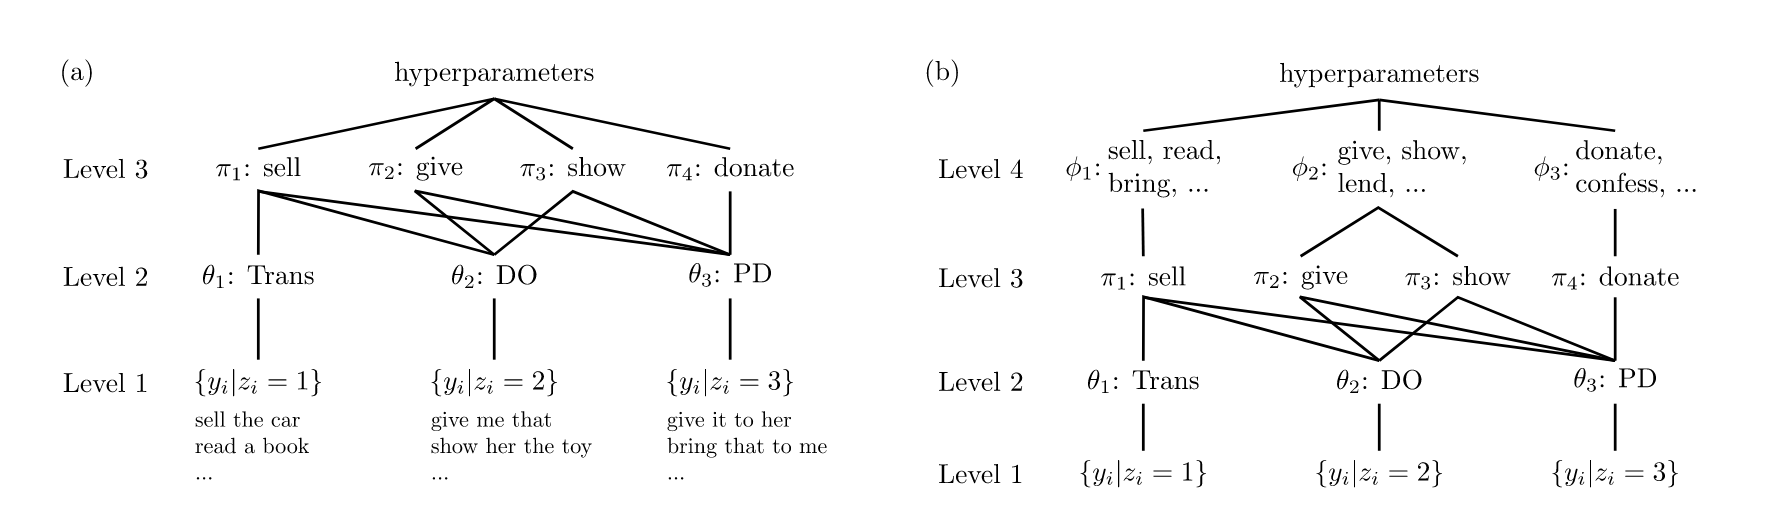
\includegraphics[width=\textwidth]{figures/verb_alternation_classes.png}
    \centering
    \caption{(a) Model 1, a Hierarchical Dirichlet Process applied to learning verb argument structure constructions. (b) Model 2,
    an extension of Model 1 to learn verb alternation classes.}\label{fig:parisien2010}
\end{figure}

\section{Cross-lingual verb sense alignment}

A cross-lingual aligned list of counterpart verbs will be needed to compare the verb classes. The easiest way to do this is likely through existing cross-lingual word lists such as LanguageNet, part of the PanLex project \citep{kamholz2014}. However, multilingual word embeddings and induction of a cross-lingual verbal lexicon could be considered as another option should the existing resources prove insufficient.

\section{Information theory metrics}

The specific metrics to be used on the results will have to be determined in combination with the decisions to be made in the experiments such as the number of the language studied and whether parallel or non-parallel datasets are used. Preliminarily, however, information theory metrics modeled on those used by \citet{say2014} are considered, specifically an internal complexity metric measuring the entropy of the distribution of verbs among valency classes and a similarity metric based on mutual information measuring the similarity / dissimilarity between valency systems of two or more languages.
\chapter{Experiments and analysis}
\section{Experiment 1: Transitivity ratios}\label{sec:exp1}
\subsection{Background: Verb transitivity}
If we were to take a top-down approach to the task of verb classification, i.e., to categorize verbs of a language into verb classes according to their syntacto-semantic properties and behavior, we could well imagine ourselves with fine-grained verb classes à la \citet{levin1993} in the end, but will likely have to start with more basic distinctions and, first among them, that of verb \textit{transitivity}. 

In comparison with the more intricate distinctions made in valency typology, the notion of \textit{transitivity}, i.e., whether a verb can take one or more objects, is probably familiar to any of us who has been in a foreign language classroom. Traditionally, a binary distinction is made between \textit{intransitive} verbs, which take only a subject and no objects and \textit{transitive} verbs, which take one or more objects. A categorical approach would then subdivide the verbs into further categories including \textit{ditransitive} verbs (those taking two objects), ambitransitive verbs (those that can be used both transitively and intransitively), etc.

\todo{semantic aspects of transitivity}

From a functionalist perspective, however, the categorical distinctions often fail to capture other important aspects of how verbs are used. A telling early corpus-based study \citep{biber1998} touches upon this when comparing the English verbs \textit{begin} and \textit{start}. At first glance, English appears to have provided us with two verbs that are not only semantically synonymous but share valency properties as well, as they can both be used in transitive and intransitive constructions:

\begin{exe}
\ex\label{example-begin_start}
  \begin{xlist}
  \ex{I had better issue a survival kit before we \textit{start}/\textit{begin}.\\ \strut\hfill \textbf{intransitive}}
  \ex{Then they \textit{started}/\textit{began} the quota system.\\ \strut\hfill \textbf{transitive with noun phrase}}
  \ex{They'd \textit{started}/\textit{begun} leaving before I arrived.\\ \strut\hfill \textbf{transitive with \textit{-ing} clause}}
  \ex{One of the wheels had \textit{started}/\textit{begun} to wobble.\\ \strut\hfill \textbf{transitive with \textit{to} clause}}
  \end{xlist}
\end{exe}

This however belies the different usage patterns exhibited by these verbs, as \citet[95]{biber1998} demonstrate with statistics from the British National Corpus (BNC): while both uses are present for both verbs, \textit{begin} is used more often in a transitive frame than \textit{start} across different genres: in fiction, 78\% of \textit{begin} occurrences (196/250) are with various transitive patterns vs. only 60\% for \textit{start} (149/250); transitive uses are less frequent in academic texts in general but the observation of relatively higher transitivity for \textit{begin} still holds (57\% vs. 36\%, or 110/192 vs. 51/142).

The UD annotations provide us with good facility to investigate transitivity at a lexeme-level quantitatively, as it would allow us similar insights but with a wider range of languages and better coverage of their respective verbal lexicon. The relevant dependency relations \textsc{nsubj} and \textsc{obj} are defined to cover respectively the first and second core arguments of a verb with their typical syntactic roles as subject and object. This is defined without respect to specific cases (even though typically the accusative in languages with a case system) or semantic roles (even though they would typically be the proto-agent and proto-patient) in an effort to not prejudice the scheme with a priori categories to the extent possible. The renaming of the \textsc{dobj} relation to \textsc{obj} changes introduced by UD v2 \citep{nivre2020} reflects the same effort as well.

\subsection{Experiment design}

Given the clear and typologically sound UD dependency relations, one can be forgiven for having already started up the code editor and tried to calculate the transitivity ratio based on them. On closer examination, however, we see that arriving at a clear definition of transitivity is in fact not trivial.

We consider four different definitions of a quantitative transitivity ratio within the UD annotation scheme:

\begin{enumerate}
    \item the number of verb instances with both \textsc{nsubj} and \textsc{obj} dependents, divided by the number of verb instances with an \textsc{nsubj} dependent
    \item the number of verb instances with an \textsc{obj} dependent, divided by the number of verb instances with an \textsc{nsubj} dependent
    \item the number of verb instances with an \textsc{obj} dependent, divided by the total number of verb instances
    \item the number of verb instances with an \textsc{obj} dependent, divided by the number of verb instances with either an \textsc{nsubj} or an \textsc{obj} dependent
\end{enumerate}

Def. 1 is an attempt at enforcing the definition of the transitive object as the \textit{second} core argument of the verb by excluding from calculation instances where the first core argument (i.e., subject) is not realized. This turns out counterproductive for two reasons. Firstly, this does not sit well with the focus on transitivity, as instances of verb use where the subject is not expressed are not per se evidence against the fact that the verb is taking a transitive object; secondly, this is undesirable from a typological perspective as well, as the metric would be biased against pro-drop languages where the pronouns would often be dropped when inferrable from grammar or context. \todo{an example sentence from a pro-drop language to illustrate}

Def. 2 comes as a reaction to the deficiencies of Def. 1, namely by dropping the requirement in the numerator for verbs to have an \textsc{nsubj} dependent. However, we are now left with the opposite problem if we are to account for typological variations, where pro-drop languages are likely to have a smaller denominator, resulting in an undesired higher transitivity ratio. The pendular biases tempt us to simply drop the \textsc{nsubj} requirement in the denominator too, arriving at Def. 3, which appears to be an elegant and simple solution. That is, until we realize the verb instances where both subject and object are dropped would affect the denominator, and such usage, e.g., non-predicative usage of verbs, is unlikely to be equally frequent in different languages and would therefore interfere with the cross-lingual comparability of our transitivity ratio. Taking all these potential drawbacks into consideration, we propose Def. 4 with the number of verb instances with either an \textsc{nsubj} or an \textsc{obj} dependent in the denominator. 

\begin{table}[ht]
    \centering
    \begin{tabularx}{0.5\textwidth}{cX}
    {\#} & \textbf{Definition} \\
    \hline
    1&$[+\textsc{nsubj}, +\textsc{obj}]/ [+\textsc{subj}]$ \\
    2&$[+\textsc{obj}] / [+\textsc{nsubj}]$  \\
    3&$[+\textsc{obj}] / [\pm\textsc{nsubj}, \pm\textsc{obj}]$\\
    4&$[+\textsc{obj}] / [+\textsc{nsubj}] \text{ or } [+\textsc{obj}]$
    \end{tabularx}
    \caption{Potential definitions of transitivity ratio considered in §\ref{sec:exp1}, represented with feature matrices}\label{tab:transitivity-defs}
\end{table} 

While we have a strong case for Def. 4 being the most principled definition, we nevertheless implement all four definitions in this experiment to empirically verify our intuitions. They are also represented with feature matrices in Tab.~\ref{tab:transitivity-defs} for quick reference.

In the experiment, we go through all eligible UD corpora and first compile transitivity ratio statistics for each verb lexeme based on the definitions. From there, we compute the per-language statistics that will become the basis for our cross-lingual comparison: we calculate the lexeme-level and token-level transitivity ratios for each language, respectively the arithmetic mean of the lexeme transitivity ratios and the mean of lexeme transitivity ratios weighted by the frequency of the lexeme. In addition to our transitivity ratio metrics, we will also calculate an additional metric, percentage of transitive verbs, i.e., the percentage of verbs in the observed lexicon that are not strictly intransitive (defined as never observed to take an \textsc{obj}), which should correspond better with the traditional binary distinction between transitive and intransitive verbs.

\subsection{Results}

\begin{table}[ht]{}
    \centering
    \small
    \begin{tabularx}{\textwidth}{lXXX}
      \toprule
      def. & lexeme tr.,\newline token tr. & tr. verb \%,\newline lexeme tr. & tr. verb \%,\newline token tr. \\
      \midrule
      1 & $\rho(54)=.83, p=.000$ & $\rho(54)=.61, p=.000$ & $\rho(54)=.70, p=.000$ \\
      2 & $\rho(54)=.81, p=.000$ & $\rho(54)=-.17, p=.221$ & $\rho(54)=-.03, p=.817$ \\
      3 & $\rho(54)=.77, p=.000$ & $\rho(54)=.64, p=.000$ & $\rho(54)=.73, p=.000$ \\
      4 & $\rho(54)=.87, p=.000$ & $\rho(54)=.61, p=.000$ & $\rho(54)=.61, p=.000$ \\
      \bottomrule
    \end{tabularx}
    \caption{Spearman's rank correlation between the transitivity metrics}\label{tab:transitivity_spearmanr} 
\end{table}  

We perform the experiment on the selected subset of UD data as described in §\ref{subsec:data_ud}. For the analysis, we include only languages with at least 100 observed verb lexemes (56 out of 79 languages); the full results from the experiments can be found in the accompanying data and appendices. 

To compare between the different definitions of transitivity, we compute Spearman's rank correlations between the lexeme- and token-level means of transitivity ratios according to each of our four definitions, as well as between the transitive verb percentage and each of them. The correlation statistics are listed in Tab.~\ref{tab:transitivity_spearmanr}. We observe overall strong correlations between the mean transitivity ratios at lexeme- and token-levels for all four definitions, with the highest observed for definition 4 ($\rho(54)=.87, p=.000$) and lowest observed for definition 3 ($\rho(54)=.77, p=.000$). This is not surprising as we have no reason to expect the more frequent verbs to behave differently from the less frequent verbs with regard to transitivity ratios. This can be confirmed by correlation tests between verb frequency and verb transitivity ratios for each language, which show no strong correlation (the mean absolute value of the Spearman's rank correlations for the languages is 0.087).

The correlation statistics between the transitive verb percentages and the transitivity ratios are slightly more revealing, if nothing else, they help us eliminate definition 2 from the competition as it shows no statistically significant correlation ($\rho(54)=-.17, p=.221$ for lexeme-level transitivity ratios and $\rho(54)=-.03, p=.817$ for token-level) while strong correlations are observed for all three other definitions (see Tab.~\ref{tab:transitivity_spearmanr}).

In the absence of a strong empirical reason based on correlation statistics to select a definition among the remaining three over the others, we proceed with the rest of the analysis with results using def. 4, which we had considered \textit{a priori} to be the most principled.

\begin{table}[ht]
    \centering
    \small
    \begin{subtable}[c]{\textwidth}
      \centering
      \begin{tabular}{lrr|lrr}
        \toprule
        Language & \# Verbs & Tr. verb \% & Language & \# Verbs & Tr. verb \% \\
        \midrule
        Catalan & 628 & 99.2\% & Maltese & 78 & 55.1\% \\
        Galician & 341 & 97.7\% & Hebrew & 536 & 58.4\% \\
        Urdu & 69 & 97.1\% & Hungarian & 73 & 64.4\% \\
        Hindi & 207 & 97.1\% & Russian & 2583 & 65.0\% \\
        Spanish & 948 & 96.9\% & Slovak & 284 & 66.5\% \\
        Indonesian & 330 & 96.7\% & Uyghur & 93 & 66.7\% \\
        Vietnamese & 156 & 95.5\% & Coptic & 128 & 68.0\% \\
        French & 735 & 94.8\% & Old Church Slavonic & 223 & 68.6\% \\
        Gheg & 50 & 94.0\% & Polish & 1080 & 68.8\% \\
        Danish & 212 & 93.9\% & Bambara & 50 & 70.0\% \\
        English & 773 & 93.4\% & Erzya & 87 & 70.1\% \\
        Afrikaans & 119 & 93.3\% & Latvian & 794 & 71.2\% \\
        Norwegian & 765 & 92.9\% & Gothic & 201 & 73.1\% \\
        Basque & 255 & 92.9\% & Old French & 444 & 74.1\% \\
        Ancient Greek & 1127 & 92.7\% & Faroese & 117 & 74.4\% \\
        \dots & \dots & \dots & \dots & \dots & \dots \\
        \bottomrule
      \end{tabular}
      \caption{by transitive verb percentage}
      \label{tab:most_tr_by_verb_percentage}
    \end{subtable}\\
    \begin{subtable}[c]{\textwidth}
      \centering
      \begin{tabular}{lrr|lrr}
        \toprule
        Language & \# Verbs & Token tr. & Language & \# Verbs & Token tr. \\
        \midrule
        Akkadian & 76 & 75.9\% & Scottish Gaelic & 53 & 16.2\% \\
        Catalan & 628 & 75.9\% & Irish & 108 & 30.8\% \\
        Galician & 341 & 70.5\% & Maltese & 78 & 31.7\% \\
        Afrikaans & 119 & 65.3\% & Faroese & 117 & 32.6\% \\
        Urdu & 69 & 65.2\% & Japanese & 395 & 33.4\% \\
        Gheg & 50 & 64.8\% & Hebrew & 536 & 33.5\% \\
        Vietnamese & 156 & 64.8\% & Polish & 1080 & 34.0\% \\
        Thai & 77 & 64.7\% & Uyghur & 93 & 34.1\% \\
        Classical Chinese & 1192 & 63.8\% & Erzya & 87 & 36.0\% \\
        Pomak & 244 & 62.1\% & Russian & 2583 & 37.4\% \\
        Spanish & 948 & 61.1\% & Dutch & 497 & 37.5\% \\
        Hindi & 207 & 60.8\% & Latvian & 794 & 37.8\% \\
        Chinese & 380 & 60.7\% & North Sami & 76 & 38.2\% \\
        Xibe & 74 & 58.8\% & Serbian & 214 & 38.4\% \\
        Ancient Greek & 1127 & 58.5\% & Arabic & 407 & 39.7\% \\
        \dots & \dots & \dots & \dots & \dots & \dots \\
        \bottomrule
      \end{tabular}
      \caption{by token-level transitivity ratio}
      \label{tab:most_tr_by_token_mean}
    \end{subtable}
    \caption{Most and least transitive languages by different metrics}
    \label{tab:most_tr_languages}
  \end{table}

\todo{most transitive languages}
\todo{least transitive languages}
\todo{areal patterns and comparison against previous studies}

\begin{sidewaysfigure}[ht]
  \centering
  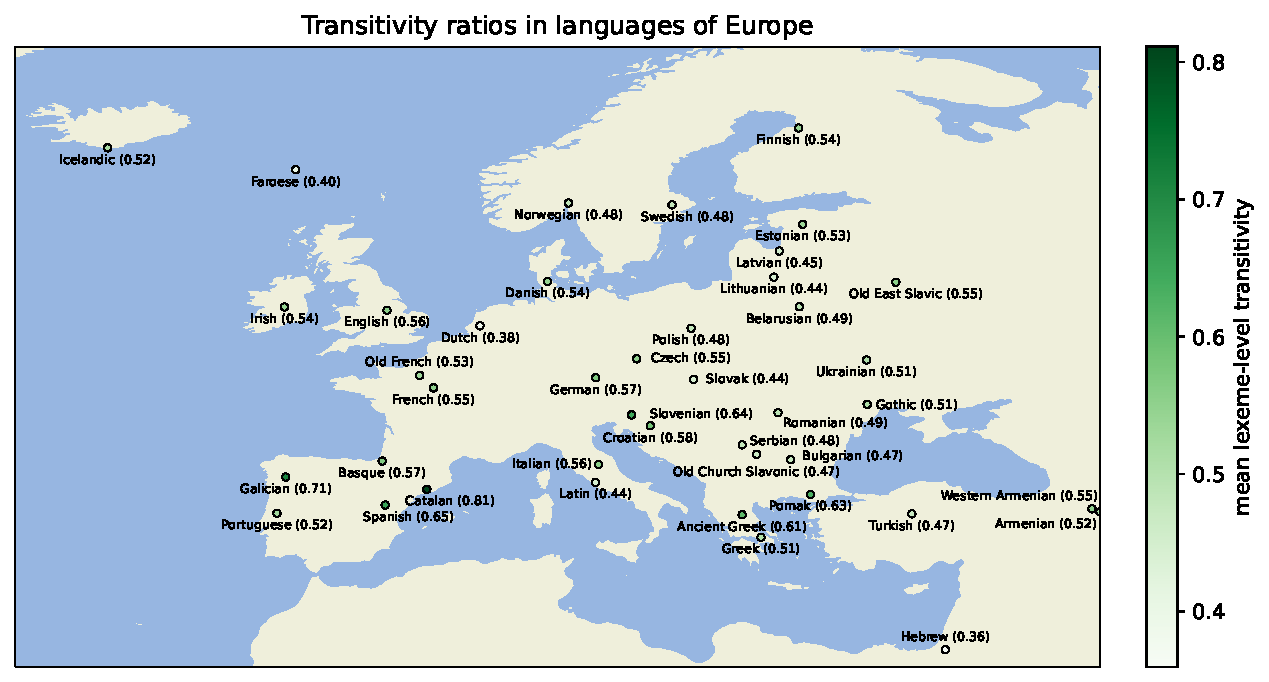
\includegraphics[width=\textwidth]{figures/transitivity_europe.pdf}
  \caption{Mean transitivity ratios in languages of Europe}
  \label{fig:transitivity_europe}
\end{sidewaysfigure}

compare results with \citet{say2014} - same areal patterns

\section{Experiment 2: Valency entropy}
\subsection{Motivation}
\subsection{Experiment design}
\subsection{Results}

\section{Experiment 3: Word order and case information}
\subsection{Motivation}
\subsection{Experiment design: ablation studies}
\subsection{Results}

\section{Experiment 4: Verb entropy}
\subsection{Motivation}
\subsection{Experiment design}
\subsection{Results}

\section{Experiment 5: Verb-finalness}
\subsection{Motivation}
\subsection{Experiment design}
\subsection{Results}
\chapter{Conclusion and outlook}\label{chapter:conclusion}

As indicated by the title, this thesis reports on several experiments on the cross-linguistic patterns in verbal valency systems. The exploratory nature of the experiments and the range of experiments make it easy to lose track of the overarching research questions. I summarize the experiments and their findings in this section, and discuss them in conjunction to how they help answer these questions. 

The two main research questions of the thesis are: (1) Do quantitative methods provide a way to characterize verbal valency and verbal valency systems in a manner that facilitates cross-lingual comparison? (2) If so, do the results allow us to draw inferences about cross-lingual differences as well as commonalities in how languages structure their verbal valency systems.

Two substantive experiments (1-2) are presented that address both research questions from different perspectives. Two additional experiments (3-4) point to possible future directions of work. 

Experiment 1 starts with a more basic measure for one aspect of valency, i.e. transitivity. Using corpus-based and quantitative versions of the transitivity ratio metric, it shows a general but not inviolable common tendency of languages to structure their verbal lexicon towards both ends of the transitivity spectrum, and show that the metric indicates areal and genetic patterns of transitivity between languages. Experiment 2-4 expands the scope of investigation and use information-theoretic metrics of valency frame entropy as a more holistic characterization of verbal valency. Correspondingly, linguistic differences and universals are explored with hypotheses motivated by cognitive linguistics approaches, taking learnability and efficiency constraints on language structure into account.

The results from the experiments support the view that how languages organize their verbal valency systems as well as the parts of verbal lexicon and grammar that are relevant shares cross-linguistic similarities shaped by common constraints but also shows differences in the different strategies they employ. It is relatively neutral in terms of lexeme- vs. frame-based view of valency but results from experiment 4 also suggests that the two views may not be irreconcilable with different languages leveraging different parts of the grammar to achieve the same communicative goals.

\section{Note on reproducibility}
Code and results for the thesis will be made available at the following repository: \url{https://github.com/siyutao/verbal-valency-ud}


\appendix
\chapter{Experiment 1 Results}
\section{Per language transitivity statistics}
\begin{longtable}{lrrrr}
    \toprule
    language name & total & tr verb percent & 4 mean & 4 weighted mean \\
    \midrule
    \endfirsthead
    \toprule
    language name & total & tr verb percent & 4 mean & 4 weighted mean \\
    \midrule
    \endhead
    \midrule
    \multicolumn{5}{r}{Continued on next page} \\
    \midrule
    \endfoot
    \bottomrule
    \endlastfoot
    Akkadian & 45 & 62.22\% & 73.38\% & 80.32\% \\
    Armenian & 227 & 70.48\% & 51.53\% & 48.98\% \\
    Welsh & 17 & 70.59\% & 35.53\% & 9.45\% \\
    Gheg & 50 & 86.00\% & 65.95\% & 64.82\% \\
    Norwegian & 765 & 89.67\% & 48.30\% & 44.80\% \\
    Old East Slavic & 500 & 65.80\% & 55.43\% & 48.87\% \\
    English & 771 & 88.72\% & 55.51\% & 52.90\% \\
    French & 733 & 90.86\% & 55.15\% & 51.29\% \\
    Slovenian & 514 & 79.57\% & 64.30\% & 55.55\% \\
    Hebrew & 531 & 51.98\% & 35.94\% & 33.50\% \\
    Kurmanji & 21 & 52.38\% & 27.94\% & 38.02\% \\
    Italian & 921 & 82.41\% & 55.70\% & 54.50\% \\
    Turkish & 773 & 73.74\% & 47.20\% & 48.54\% \\
    Finnish & 682 & 69.94\% & 53.94\% & 48.41\% \\
    Indonesian & 330 & 91.21\% & 49.74\% & 51.21\% \\
    Ukrainian & 228 & 66.23\% & 50.64\% & 45.33\% \\
    Dutch & 497 & 75.65\% & 38.10\% & 37.51\% \\
    Polish & 1059 & 61.95\% & 47.67\% & 34.07\% \\
    Portuguese & 1203 & 77.47\% & 52.46\% & 52.45\% \\
    Kazakh & 30 & 63.33\% & 45.43\% & 39.91\% \\
    Latin & 1143 & 72.35\% & 44.50\% & 40.85\% \\
    Old French & 422 & 70.14\% & 52.96\% & 53.50\% \\
    Spanish & 941 & 92.88\% & 65.36\% & 61.08\% \\
    Buryat & 27 & 51.85\% & 35.67\% & 36.83\% \\
    Icelandic & 997 & 86.56\% & 51.81\% & 41.05\% \\
    Estonian & 672 & 67.71\% & 53.48\% & 49.69\% \\
    Croatian & 386 & 84.97\% & 58.34\% & 50.27\% \\
    Gothic & 195 & 58.46\% & 50.92\% & 45.80\% \\
    North Sami & 75 & 76.00\% & 49.35\% & 37.91\% \\
    Naija & 200 & 88.50\% & 54.92\% & 45.43\% \\
    German & 1998 & 89.69\% & 57.18\% & 56.84\% \\
    Latvian & 787 & 63.79\% & 45.18\% & 37.71\% \\
    Chinese & 369 & 83.74\% & 60.56\% & 62.90\% \\
    Irish & 107 & 77.57\% & 54.22\% & 30.87\% \\
    Xibe & 62 & 70.97\% & 65.22\% & 58.37\% \\
    Bambara & 50 & 62.00\% & 54.14\% & 43.08\% \\
    Lithuanian & 212 & 58.02\% & 44.38\% & 41.48\% \\
    Galician & 339 & 88.79\% & 71.14\% & 70.44\% \\
    Vietnamese & 150 & 84.00\% & 62.00\% & 64.25\% \\
    Greek & 145 & 77.24\% & 50.65\% & 48.68\% \\
    Catalan & 627 & 98.25\% & 81.12\% & 75.86\% \\
    Swedish & 391 & 86.45\% & 47.79\% & 46.49\% \\
    Russian & 2558 & 59.34\% & 43.43\% & 37.35\% \\
    Czech & 2083 & 72.88\% & 54.72\% & 46.76\% \\
    Erzya & 87 & 54.02\% & 40.36\% & 36.01\% \\
    Thai & 69 & 69.57\% & 51.99\% & 63.16\% \\
    Basque & 249 & 78.71\% & 56.54\% & 54.51\% \\
    Slovak & 279 & 55.91\% & 44.26\% & 42.32\% \\
    Tamil & 41 & 80.49\% & 50.32\% & 42.73\% \\
    Maltese & 67 & 43.28\% & 30.35\% & 27.34\% \\
    Ancient Greek & 1111 & 81.55\% & 60.97\% & 58.47\% \\
    Ancient Hebrew & 89 & 73.03\% & 53.43\% & 48.40\% \\
    Mbya Guarani & 5 & 60.00\% & 57.33\% & 51.46\% \\
    Urdu & 69 & 85.51\% & 62.27\% & 65.23\% \\
    Romanian & 1002 & 79.84\% & 48.65\% & 48.86\% \\
    Persian & 308 & 72.73\% & 54.05\% & 50.27\% \\
    Japanese & 381 & 61.15\% & 50.06\% & 33.54\% \\
    Hungarian & 73 & 60.27\% & 44.39\% & 40.16\% \\
    Hindi & 202 & 83.66\% & 61.24\% & 60.74\% \\
    Classical Chinese & 1166 & 79.42\% & 60.76\% & 63.84\% \\
    Faroese & 114 & 71.93\% & 40.13\% & 32.51\% \\
    Sanskrit & 106 & 74.53\% & 57.49\% & 51.74\% \\
    Arabic & 407 & 72.48\% & 46.74\% & 39.65\% \\
    Wolof & 155 & 87.10\% & 55.11\% & 53.52\% \\
    Bulgarian & 348 & 81.32\% & 47.10\% & 47.64\% \\
    Cantonese & 45 & 73.33\% & 55.92\% & 50.99\% \\
    Pomak & 229 & 72.49\% & 63.20\% & 61.76\% \\
    Old Church Slavonic & 211 & 54.50\% & 46.60\% & 43.49\% \\
    Upper Sorbian & 10 & 70.00\% & 40.82\% & 38.59\% \\
    Danish & 212 & 88.68\% & 54.47\% & 51.92\% \\
    Komi Zyrian & 25 & 32.00\% & 28.64\% & 25.52\% \\
    Manx & 25 & 72.00\% & 47.98\% & 22.92\% \\
    Afrikaans & 117 & 82.91\% & 60.90\% & 65.13\% \\
    Belarusian & 587 & 68.14\% & 49.27\% & 44.41\% \\
    Coptic & 127 & 65.35\% & 41.30\% & 43.55\% \\
    Serbian & 214 & 73.36\% & 47.94\% & 38.45\% \\
    Western Armenian & 299 & 75.92\% & 54.87\% & 50.66\% \\
    Scottish Gaelic & 53 & 77.36\% & 37.74\% & 16.17\% \\
    Uyghur & 80 & 53.75\% & 37.84\% & 32.95\% \\
\end{longtable}
    

\backmatter

% optional: list of figures, list of tables
% \listoffigures
% \listoftables

\chapter{Bibliography}
\printbibliography[heading=none]

\end{document}
